
\documentclass[a4paper,11pt,twoside]{article}
\author{Ian J. Lewis}
\date{\today}
\title{Fprolog, adding functions to Prolog via a mainstream approach}

\hyphenation{Fprolog}

\newcommand{\todo}[1]{\vbox{
                            \hrule 
                            \hbox{\strut \vrule{} {\textbf{todo:} #1} \vrule}
                            \hrule 
                           }}


%\renewcommand{\topfraction}{.8}
%\renewcommand{\bottomfraction}{.8}
%\renewcommand{\textfraction}{.2}
%\renewcommand{\floatpagefraction}{.8}
%\renewcommand{\baselinestretch}{1.1}
\setlength{\parindent}{0pt}
%\setlength{\parskip}{3pt}

% This is to change the width of a page
%\textwidth 15.3cm


\def\postscript{{\sc postscript}}
%\input{psfig}

%\psfull

\usepackage{rotating}
\usepackage{subfigure}
\usepackage{latexsym}
\usepackage{alltt}
\usepackage{graphicx}

\begin{document}

\huge
\noindent
{\bf Distributed logic programming with oracles and \texttt{kappa}}
\normalsize
\\
\\
\large
\noindent {\bf Ian J. Lewis}\\
University of Cambridge\\
Cambridge, England, CB2 3QG\\
\\

\Large
\noindent
{\bf Abstract}
\normalsize
\\

\noindent
The recursive backtracking performed during the execution of a Prolog program can
be interpreted as the traversal of a proof tree.  An \textit{oracle} is a sequence
of clause indexes representing a path within that tree.  Combined with the depth-first
left-to-right search of standard Prolog, an oracle provides an effective means of
communicating and recreating
the state of an interrupted processor, denoting a subtree for search, uniquely
identifying a returned solution, and dividing the search tree into two parts.  This
paper shows how those properties can be exploited in a simple yet effective OR-parallel
Prolog system for distributed networks of general purpose workstations.

%%%%%%%%%%%%%%%%%%%%%%%%
\section{Introduction} %
%%%%%%%%%%%%%%%%%%%%%%%%

Given a goal clause and a program, a Prolog system will systematically
search the implied AND-OR
proof tree.  OR-parallel systems evaluate alternative choices in parallel, generally
requiring the accumulated state to be communicated or shared among the processors
working within a common subtree \cite{Ali87, B+92, Clo92, DLO87, LWH+90, War87}.
The use of oracles, proposed by Clocksin in \cite{Clo87}, provides a model for
OR-parallel execution of logic programs in which no computation state (meaning
constructed data structures and variable bindings) need be copied or referenced between
processors.  An \textit{oracle} is a list of clause indexes defining a path in
the transformed OR-only search tree of the program.  The principle is illustrated
in the sample program given in Figure \ref{and_or_tree}, producing the
AND-OR tree represented on the right.
The left-to-right
ordering of the conjunctive goals in the body of the first clause leads to the
transformation of the AND-OR tree into the OR-only tree of Figure \ref{or_only_tree},
in which the subtree representing each conjunctive subgoal is replicated under each
terminal node of the left-most OR-only subtree.  The execution of the Prolog
program equates to the depth-first left-to-right traversal of this OR-only tree.
In this paper, \textit{search tree} will be taken to mean the
idirected acyclic graph represented by this OR-only tree.

\begin{figure}
  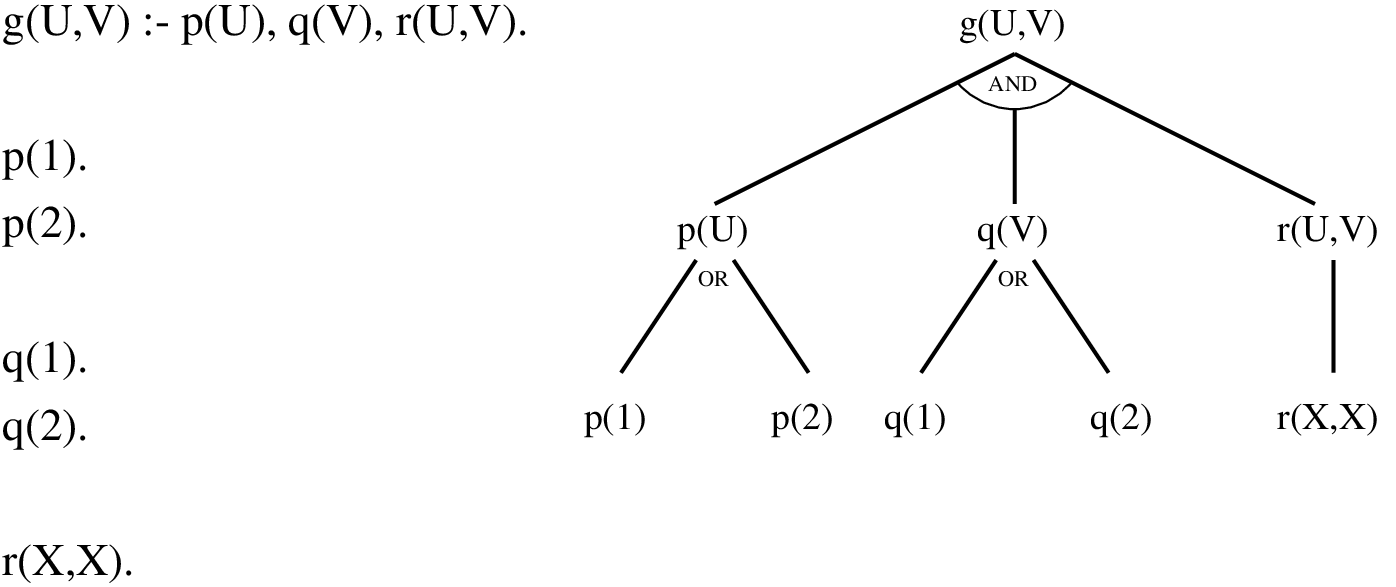
\includegraphics[width=\linewidth]{and_or_tree.png}
  \caption{AND-OR search tree for goal clause g(U,V).}
  \label{and_or_tree}
\end{figure}

Each clause of the program can be assigned an index local to its procedure, and
each oracle is a list of these indexes representing a path
from the root of the search tree.
The principle of the DelPhi machine investigated by Clocksin
and others \cite{Clo87, Sar95, Lew98} is that these paths can be articulated by
one processor for execution by others, resulting in parallel search.  Rather
than the communication or sharing of data structures created during the execution
of the program, \textit{recomputation} is used to create the bindings valid for
the assigned path.  In practical situations, it is often more efficient to use
computing cycles to recreate the environment at a given node in the search tree
than to copy or share that environment between processors.

\begin{figure}
  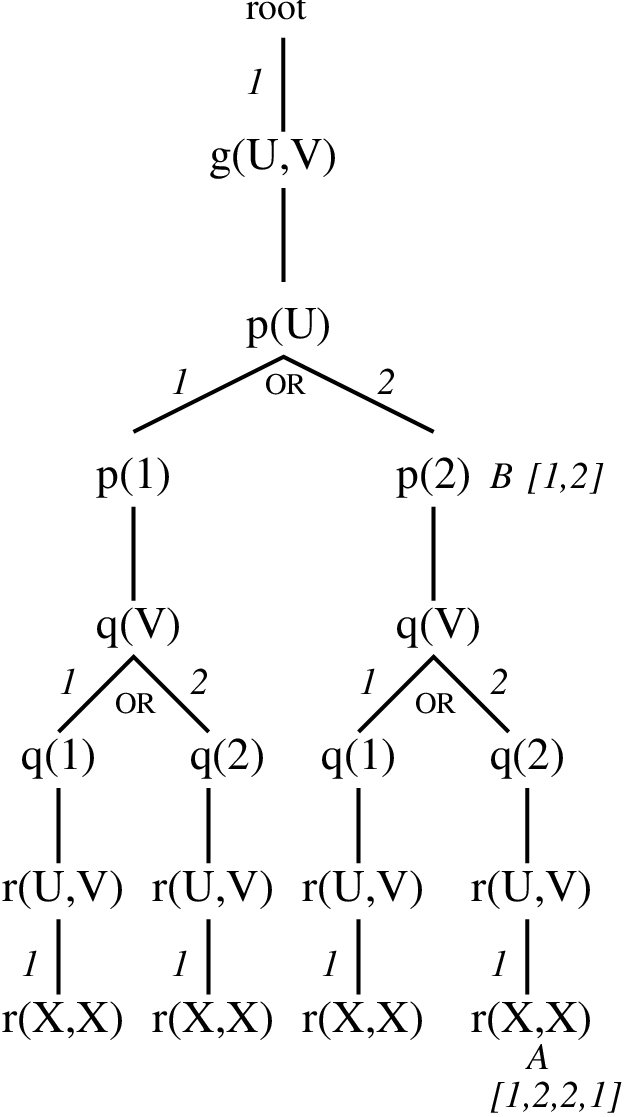
\includegraphics[width=\linewidth]{or_only_tree.png}
  \caption{OR-only tree annotated with oracle indexes.}
  \label{or_only_tree}
\end{figure}

The OR-only tree in Figure \ref{or_only_tree} is annotated with the local clause
indexes\footnote{Alternatively, the use of global clause
indexes in an oracle, such as the entry-points of each
clause, allows oracles to be followed efficiently but may be less suited to
techniques involving oracle generation outside of the program.
The use of bit strings for oracles, suggested by Clocksin in \cite{Clo87, Clo92}, is 
most suited to these approaches.}
and two oracles are illustrated.  An \textit{open oracle} defines
a path leading to an intermediate node in the search tree, such as the
oracle \textit{[1,2]} leading to the node labelled \textit{B} in the
example.  The oracle leading to the solution at the terminal node 
\textit{A} is \textit{[1,2,2,1]}.
The processor receiving the oracle is called a
\textit{path processor}, and can be expected to execute and possibly extend
the assigned oracle, communicating success or failure or returning a number
of discovered open oracles.
During execution, a path processor can maintain a
list of clause indexes leading to its current point in the search tree, this list
being its \textit{current oracle}.

The DelPhi principle permits a wide range of distributed execution strategies,
discussed in detail in \cite{Clo87, Sar95, Lew98}.  With strategies based
upon oracle generation and testing,
each path processor can limit its search along the assigned path, reporting success,
failure, or open.  Other strategies can require the path processors also extend
the assigned oracle by one or more indexes, or as with breadth-first partitioning
described below, fully search the subtree referenced by the oracle.

Thus oracles can be given a number of interpretations:
\begin{itemize}
\item{An oracle defines a path in the OR-only search tree that can be executed
  by a processor, returning success, failure, or open.  This interpretation is
  useful for parallelisation strategies using a control processor to
  generate oracles for execution by dependent path processors.}
\item{An oracle uniquely defines a node within the search tree.  For a 
  terminal node indicating success, the oracle uniquely identifies the
  solution.  The communication of work using oracles provides straightforward
  support for efficient recovery in the event of the loss of a path processor, and
  the labelling of solutions with their associated oracle permits the
  efficient reassignment of the affected work avoiding the possibility of
  duplicate solutions.}
\item{An open oracle uniquely defines the root of subtree within the search tree,
  suggesting the strategy of breadth-first partitioning in which all the
  subtrees defined by open oracles of a fixed length are allocated to the
  available path processors for distributed search.  This strategy is
  described in Section \ref{bfp_section}.}
\item{When combined with the depth-first left-to-right search strategy of standard
  Prolog, an oracle divides the OR-only search tree into a left-part and a
  right-part.  The current oracle of a busy path processor assigned a subtree
  for search divides that subtree into the parts already searched and yet to be
  searched.}
\end{itemize}

The assignment of oracles to path processors for
interpretation as references to unique subtrees for distributed search leads
to the concept of \textit{poisoned oracles}
which can greatly reduce the efficiency of simple scheduling
strategies.  For example,
a lengthy oracle leading to a
very small subtree will cause a path processor to perform much recomputation
culminating in relatively little useful work searching the allocated subtree.
Equally,
an oracle leading to a huge subtree in a strategy in which the path processor
fully searches each assigned subtree without interruption will also limit
the parallelisation efficiency.

The breadth-first partitioning (BFP) strategy described below provides effective
parallelism for programs without greatly imbalanced search trees.  The OR-parallel
partitioning can be achieved with an extra-logical predicate of only 4 lines of 'C'.
For problems with less evenly distributed work, the work splitting strategy described in
Section \ref{work_splitting} recursively applies BFP,  avoiding the inefficiency caused
by large poisoned oracles.

%%%%%%%%%%%%%%%%%%%%%%%%%%%%%%%%%%%%%%
\section{Breadth-First Partitioning} %
%%%%%%%%%%%%%%%%%%%%%%%%%%%%%%%%%%%%%%
\label{bfp_section}

The breadth-first partitioning (BFP) strategy, first 
investigated by Saraswat in \cite{Sar95}, is illustrated in
Figure \ref{bfp}.  The strategy uses the depth-first left-to-right
search of standard Prolog, proceeding in two phases:
\begin{enumerate}
\item{\textbf{Discovery of open oracles:} the search is limited to a
  specified depth limit $L$.  All the open oracles found at this depth
  are accumulated into an oracle stack for allocation in the second
  phase.  In Figure \ref{bfp} the five discovered open oracles are
  labelled A\ldots E.}
\item{\textbf{Selected subtree search:} for each oracle, a path
  processor follows the oracle and fully searches the referenced
  subtree.  With the count of path processors in the group $G$,
  each path processor is allocated a unique processor $N$ in the
  range $0\ldots G-1$.  The filter $i \mbox{ mod } G = N$ is used
  to select the $i$th oracle for execution by path processor $N$.
  In the example of Figure \ref{bfp},  a system with two path processors
  numbered $0$ and $1$ will allocate oracles B and D to processor $0$,
  and oracles A,C and E to processor $1$.}
\end{enumerate}

\begin{figure}
  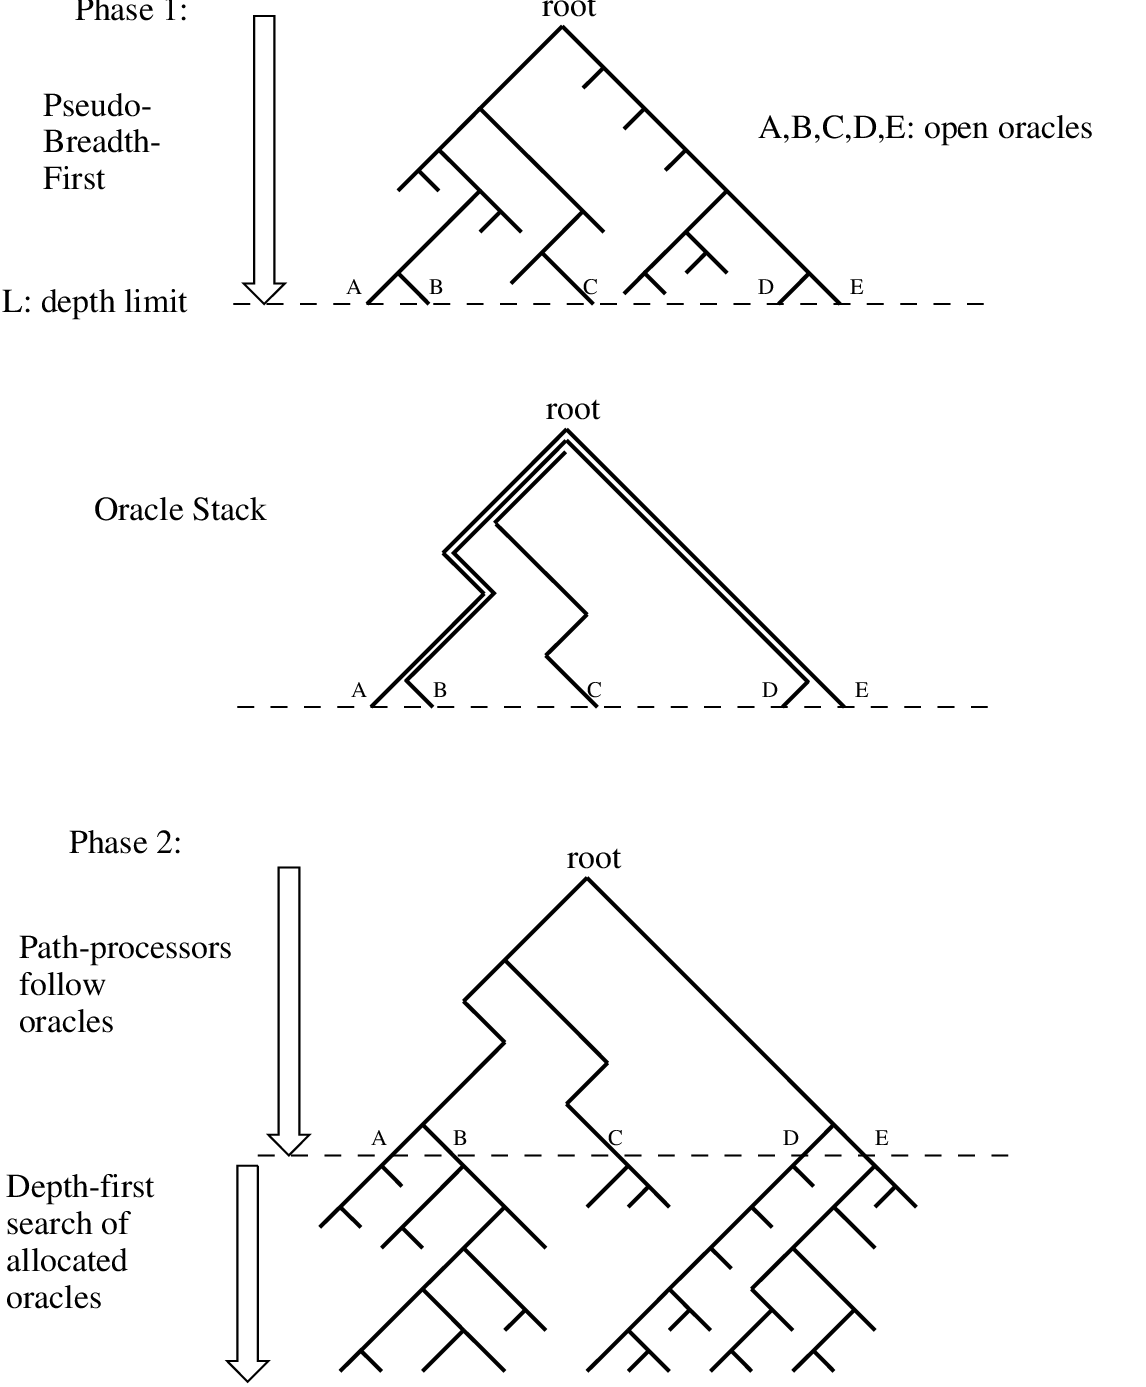
\includegraphics[width=\linewidth]{bfp.png}
  \caption{Oracles and Breadth-First Partitioning.}
  \label{bfp}
\end{figure}

The description given above suggests the generation of the oracles
in a control processor, and the 
subsequent distribution of those oracles to
the available path processors.
Communication within the system can be reduced if the oracles are
produced locally within each path processor, which then use the
$G$ and $N$ parameters to select the subtrees for local search.  A
control processor is needed to start the processes with the correct
parameters, collect the solutions, and report completion.

A number of benchmarks have been used to evaluate the performance of
the BFP strategy, with detailed results in \cite{Sar95, Lew98}.  
A series of runs of the Pentominoes program
\cite{Lew98} gives the speedup for $G=1\ldots 30$ 
in Figure \ref{pent_bfp}.  The single cpu runtime for the
Pentominoes program is 446 seconds, with the maximum improvement
reducing that time to approximately 37 seconds.  The overhead of the
oracle management
with a simple implementation increases the single-cpu runtime
by 9\% compared to the underlying standard Prolog
compiler.

\begin{figure}
  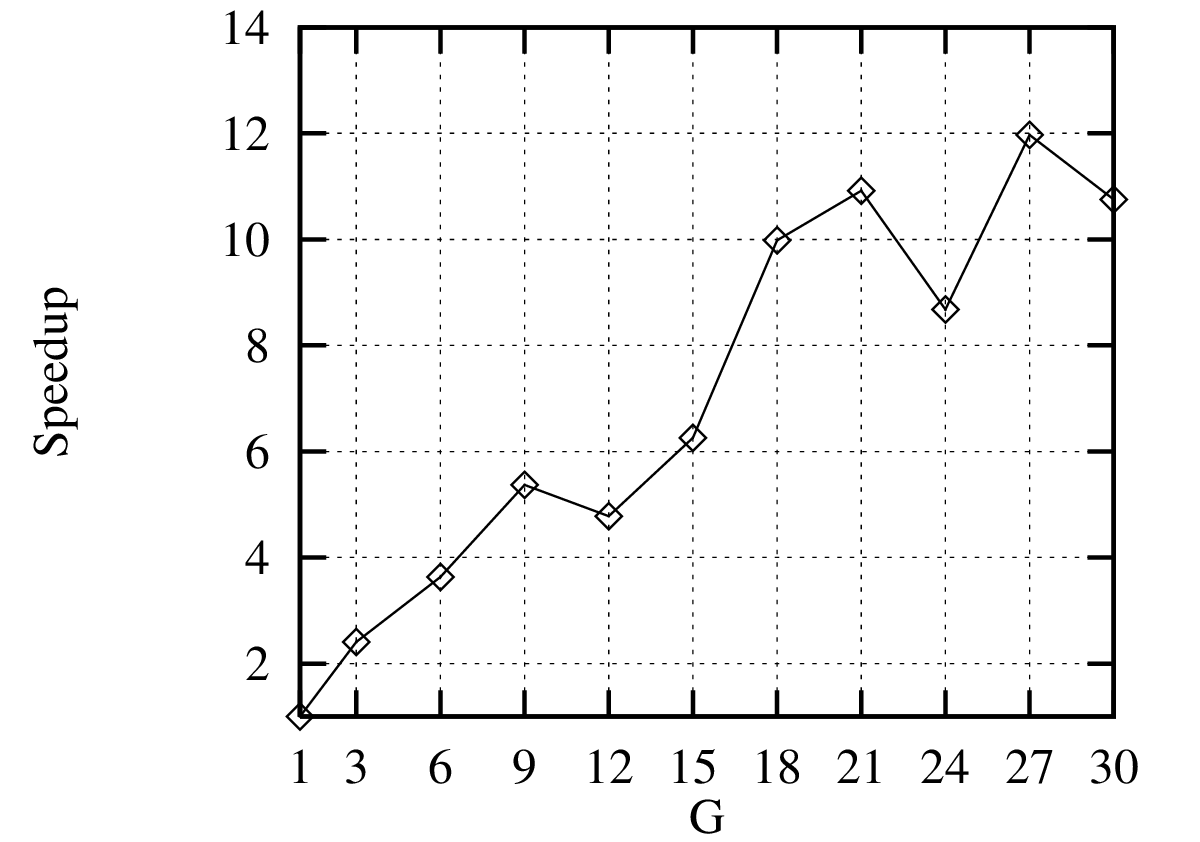
\includegraphics[width=\linewidth]{pent_bfp.png}
  \caption{Speedup achieved for Pentominoes program.}
  \label{pent_bfp}
\end{figure}

The graph for the Pentominoes problem shows a general speedup, but
reveals some issues not apparent with some more benign benchmarks,
such as N-queens.
For some group sizes, the speedup achieved for the sample problem
was less than that achieved with fewer processors ($G=12, 24$ and $30$).
This phenomenon is caused by the uneven distribution of the work
in the subtrees beneath the open oracles found at the selected
depth limit $L=21$.  At this depth limit, the Pentominoes problem
has 848 open oracles, such that the largest group of 30 processors
are assigned 28 or 29 open oracles each.  The work allocated to the
path processors benefits from averaging across the oracles assigned,
but the allocation formula includes no estimate of the work in each
subtree and some distributions may select several large subtrees for
execution by a single path processor.  In the Pentominoes problem and
other benchmarks evaluated, typically fewer than 10\% of the open
oracles referred to over 90\% of the work.  The depth limit selected
must assign enough oracles to each path processor so that all those with
small subtrees can be quickly searched.  The depth limited search of
the first phase is effectively sequential, so the limit $L$ must not be
so large as to cause the first phase to dominate the overall runtime.

\begin{figure}
  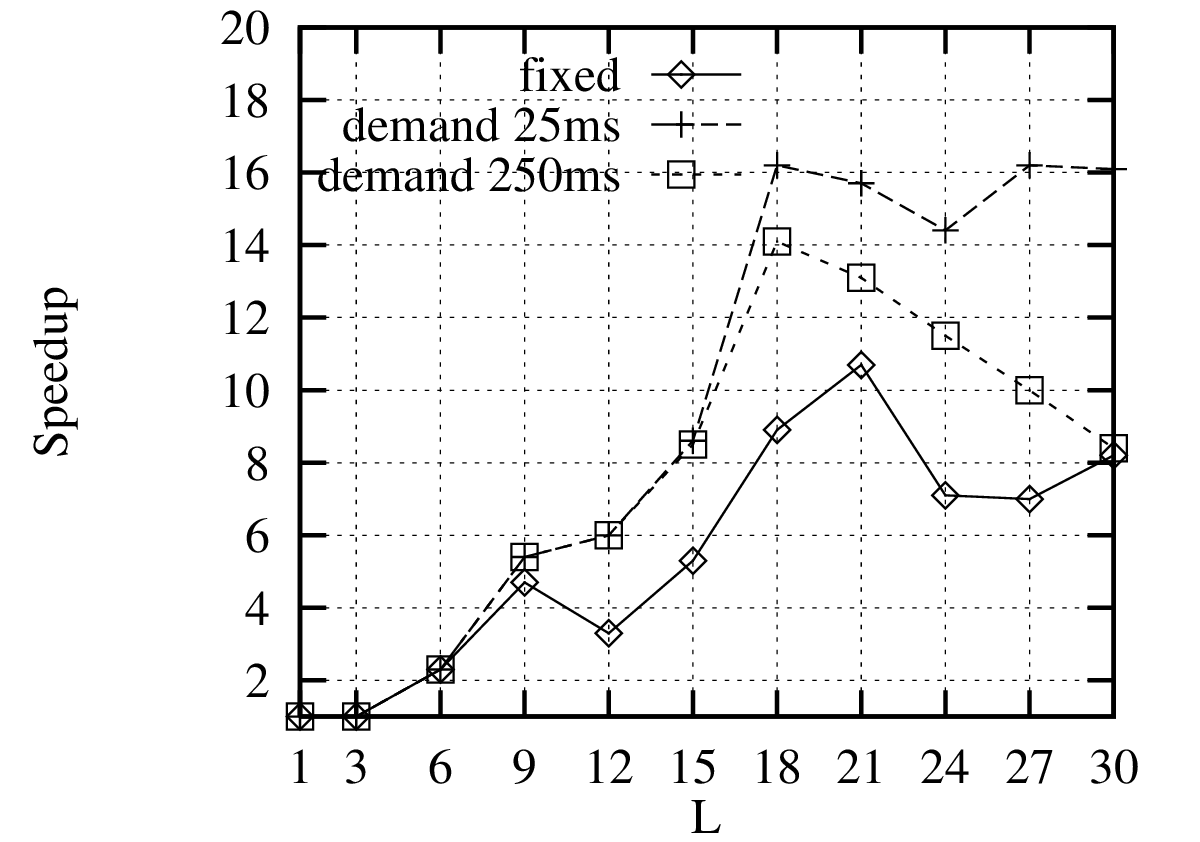
\includegraphics[width=\linewidth]{pent_bfp_l.png}
  \caption{Effect of BFP depth limit on speedup.}
  \label{pent_bfp_l}
\end{figure}


Figure \ref{pent_bfp_l} shows the speedup achieved for the 
Pentominoes program with the BFP strategy for a fixed processor
group size $G=30$, with a range of values for the partitioning
depth limit $L$ and the fixed modulo oracle allocation formula.
For small values of $L$ the speedup is limited by the small number
of oracles discovered, such that some path processors receive none.
At values of $L>21$, the overhead of the first phase reduces the
parallel speedup.  The dashed lines in the graph of Figure \ref{pent_bfp_l}
give the
speedup performance for BFP implemented with a demand-based oracle
allocation algorithm rather than the local fixed modulo formula.
This technique benefits from a more balanced allocation of the
work available at the selected depth limit, but the communication
required for the transmission of each oracle for execution
introduces a new overhead.  The graph of Figure \ref{pent_bfp_l}
shows the calculated speedups for demand-based oracle assignment,
with communication latencies of
25ms and 250ms.

\begin{figure}
  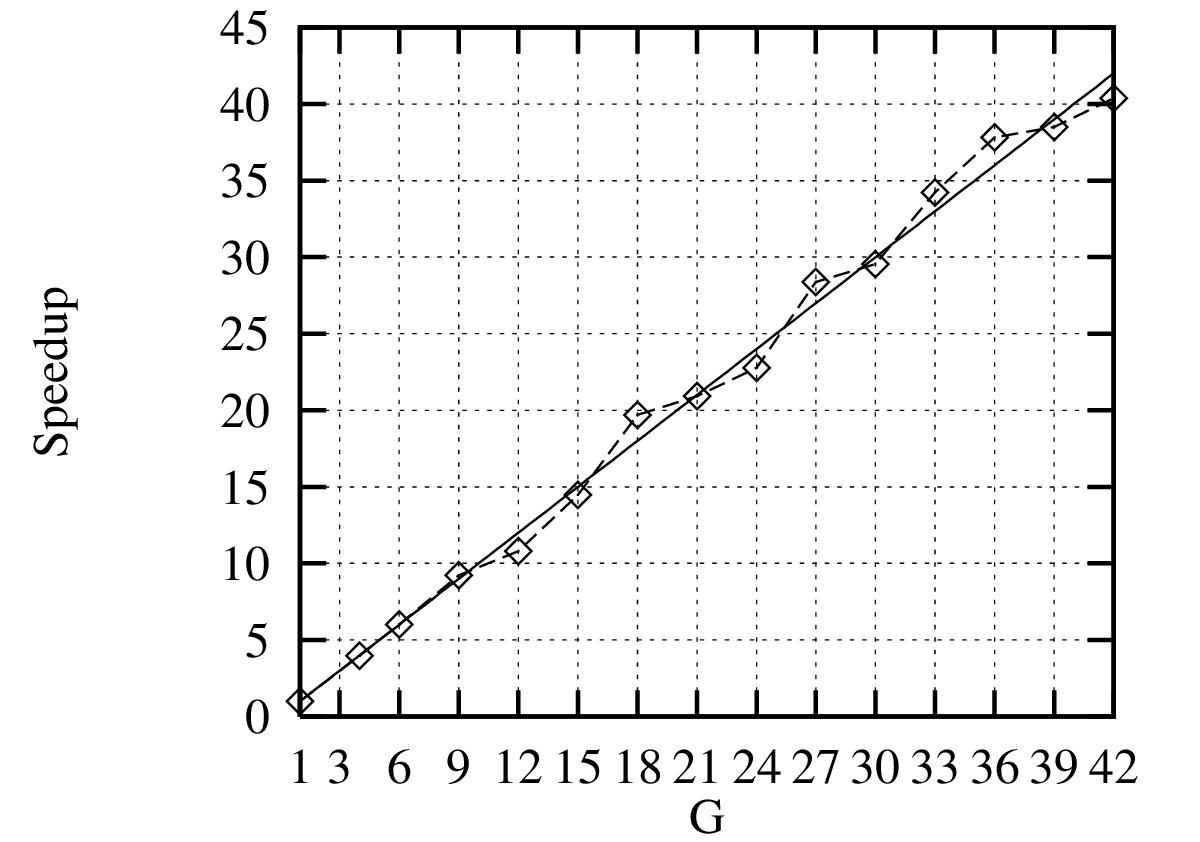
\includegraphics[width=\linewidth]{overbeek_bfp.png}
  \caption{Speedup achieved for PTTP Overbeek example 4.}
  \label{overbeek_bfp}
\end{figure}

The breadth-first partitioning strategy described above is
vulnerable to large imbalances in the work beneath each discovered
open oracle, and requires the user selection of a partitioning depth
limit.  However, with these limitations some useful results are
possible.  Figure \ref{overbeek_bfp} gives the speedups achieved
for $1\ldots 42$ processors for the Prolog Technology Theorem
Prover developed by Stickel
given a problem from Overbeek \cite{Sti88}.  The single-cpu runtime for the
program was 6 hours and 6 minutes.  The following section
describes \texttt{kappa}, a four-line extra-logical predicate which
was added to PTTP to produce the results shown.

%%%%%%%%%%%%%%%%%%%%%%%%%%%%%%%%%%%%%%%%%%%%%%%
\section{Kappa: partitioning without oracles} %
%%%%%%%%%%%%%%%%%%%%%%%%%%%%%%%%%%%%%%%%%%%%%%%
\label{kappa_section}

The two phases of the breadth-first partitioning strategy given
in Section \ref{bfp_section} with the fixed modulo oracle assignment
formula can be combined into one.  Each path processor is given the
program and the parameters $G$, $N$ and $L$, and searches from the
root to the depth limit $L$.  Oracles are not accumulated, but
a cumulative count is recorded of the number of times the depth limit
is reached.  This count is equal to the corresponding oracle number,
and the modulo selection formula can be used to identify the
subtrees which should be selected for search.  The path processor
searches each selected subtree as soon as its root is discovered
during the depth limited search.

\begin{figure}
  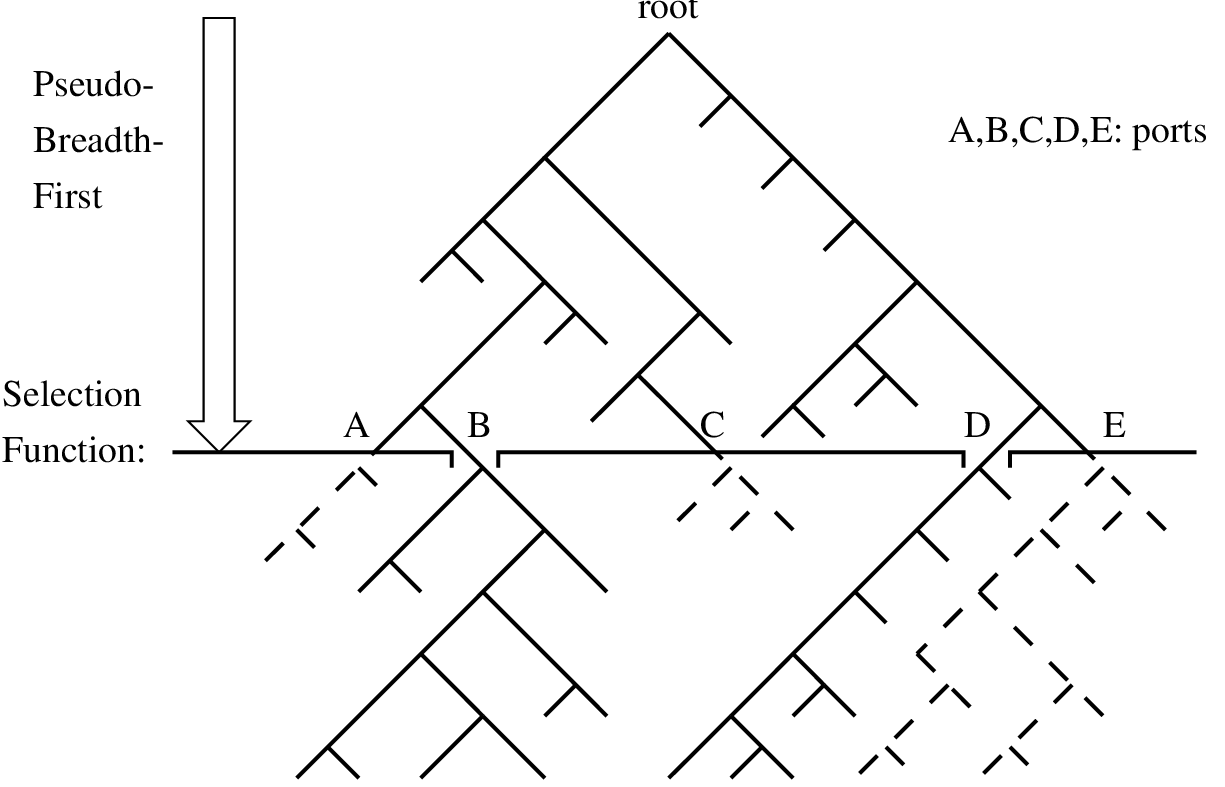
\includegraphics[width=\linewidth]{port_tree.png}
  \caption{Breadth-first partitioning without oracles.}
  \label{port_tree}
\end{figure}

The process is illustrated in Figure \ref{port_tree}, with the roots of the
subtrees at the depth limit $L$ labelled A,B,C,D and E as with the equivalent
oracles for BFP.  No oracles are used for partitioning, and the nodes in the
search tree at the depth limit $L$ at which further search is possible are
called \textit{ports}.  The resulting distributed search has much in common
with BFP, but the recomputation of the search tree beneath the depth limit is
reduced and no storage or communication resources are required for the oracles.

The partitioning can be achieved with the use of a simple extra-logical
predicate \texttt{kappa}, the source for which is
given in Section \ref{implementation}.  If one-time
partitioning is used as with BFP, the distributed program will have the
same vulnerability to ports or oracles leading to huge subtrees,
and a reasonable partitioning depth limit must be used.

The provision of 
one-time breadth-first partitioning through the introduction of the simple
extra-logical proposition \texttt{kappa} allows rapid experimentation with
OR-parallelism for existing Prolog programs.  The proposition can be automatically
added to every clause, or the programmer can annotate just one procedure.

%%%%%%%%%%%%%%%%%%%%%%%%%%%%%%%%%%%%%%%%%%%%%%%%%%%%%%%%%%
\section{Work splitting with oracles and \texttt{kappa}} %
%%%%%%%%%%%%%%%%%%%%%%%%%%%%%%%%%%%%%%%%%%%%%%%%%%%%%%%%%%
\label{work_splitting}

The strategy of breadth-first partitioning using oracles, or the similar
distributed behaviour produced through the use of \texttt{kappa}, can provide
good speedup for programs with reasonably balanced search trees.
The integration of the support for oracles into the partitioning predicate
\texttt{kappa} broadens the range of programs for which the parallelising
technique is effective.

\begin{figure}
  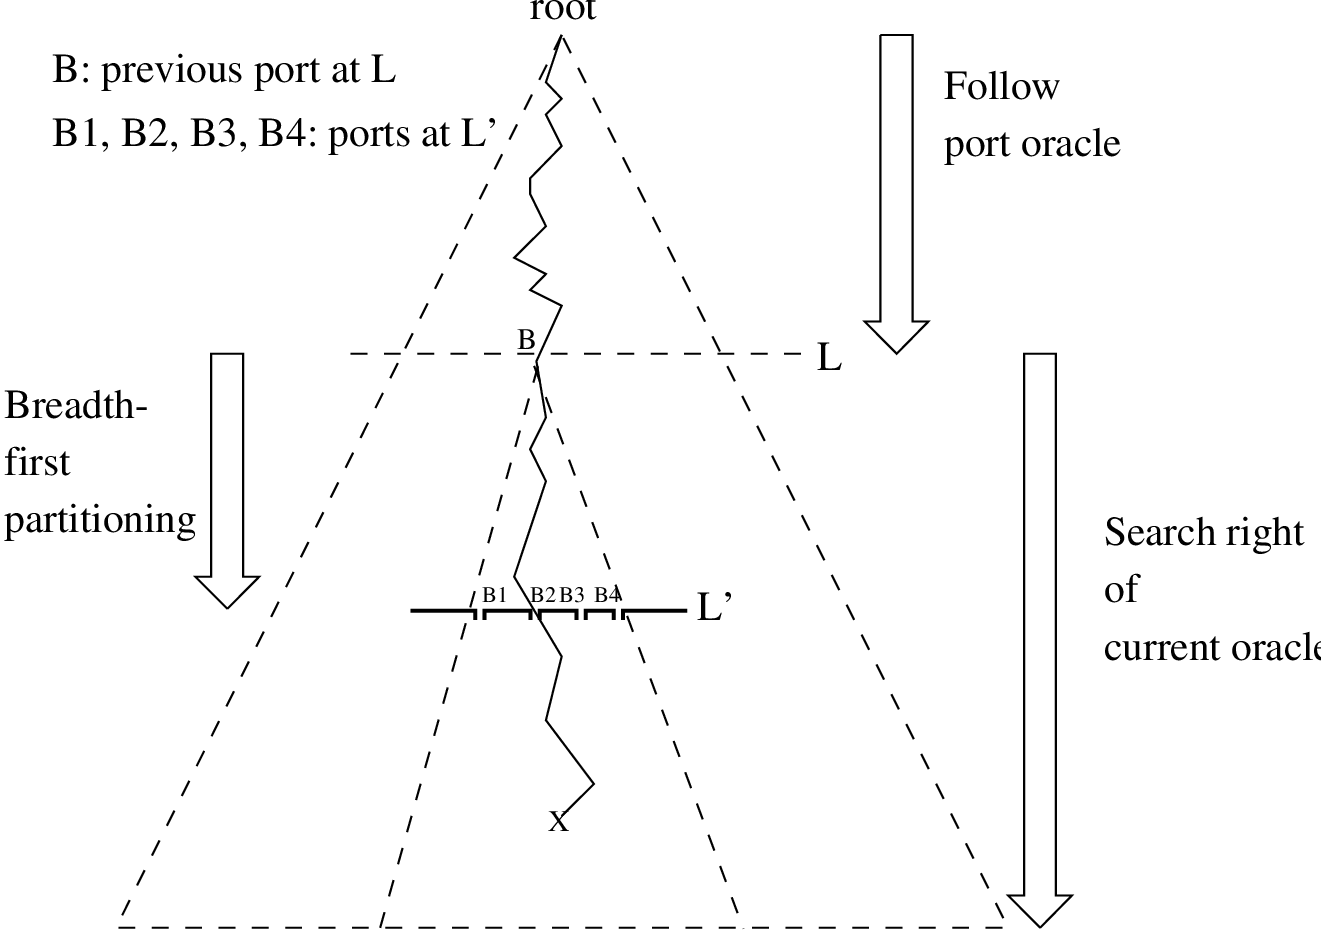
\includegraphics[width=\linewidth]{sok.png}
  \caption{Work splitting.}
  \label{sok}
\end{figure}

A graphical representation of the recursive partitioning technique, called
splitting with oracles and \texttt{kappa} (SOK), is given in Figure \ref{sok}.
Each path processor loads the user program on startup, and the assignment of
work to each path processor is specified with:
\begin{itemize}
\item{An oracle and a prefix length $L$.
  The first $L$ indexes of the oracle lead to the root of a subtree within
  which the search is to be constrained.  The root of the subtree is labelled B
  in Figure \ref{sok}.
  The remaining indexes of the oracle from B to X, divide the subtree into
  two parts.}
\item{An incremental depth limit $L'$, at which breadth-first partitioning as described
  in Section \ref{kappa_section} is to take place.}
\item{A parameter $G$ giving the number of path processors in the group allocated to
  the subtree at B.}
\item{A unique processor number $N$.}
\end{itemize}

Each path processor will \textit{follow} the assigned oracle from the root of the
search tree to B.  The remainder of the oracle is treated as a left bound to the
search within the subtree at B. With this left bound,
breadth-first partitioning is used within the subtree, and the
discovered ports at the incremental depth limit $L'$, labelled B2, B3 and
B4 in Figure \ref{sok}, are allocated modulo $G$ to the path processors
in the new group.  The path processor with
unique processor number
$N=1$ will be allocated the first port discovered at B2, and will first search the
subtree with its root at B2 with the oracle B2-X at a left bound to the search.

While executing the search, a busy path processor is liable to be interrupted,
at which point it communicates its current oracle and current partitioning depth
limit, and aborts the search of its current subtree.  The interrupted path processor
continues its search to the right of the port at which it was interrupted\footnote{
other simple splitting strategies are possible, dividing both the current subtree of
the busy processor and reallocating the remaining subtrees at the the current depth
limit.}.

The capabilities described above provide a basis for work splitting, in which one
processor can be interrupted and its work divided between a
number of path processors forming a new group.  The
extended \texttt{kappa} parallelisation primitive permits a range of scheduling strategies, 
considering:
\begin{itemize}
\item{when interruption of a busy processor should occur,}
\item{which busy processor should be interrupted,}
\item{how many idle processors should form a new group to divide the work of an
  interrupted processor,}
\item{and specifically for the use of BFP in the extended \texttt{kappa}, the initial
  and incremental depth limit.}
\end{itemize}

A simple scheduler was created for an initial evaluation at Cambridge,
in which an interruption occurred when
the number of idle processors was three or more, and each work split
was to a new group of three path processors.  The processor selected for splitting
was that with a current partitioning depth nearest the root of the search tree, and 
the incremental depth limit was double that of the interrupted busy processor. The
initial partitioning depth was 1.  Figure \ref{pent_sok} gives the speedup performance
for a network of $1\ldots 30$ workstations with the Pentominoes problem, comparing the
recursive splitting with oracles and kappa approach with the one-time partitioning
of BFP.  As with BFP, the simple implementation of oracle support with \texttt{kappa}
increased the single-cpu runtimes by 9\% over the standard Prolog compiler.  During
the execution of the Pentominoes program with the simple scheduler described, work
splitting occurred approximately 60 times on the 30-processor network, averaging one
split of a busy path processor
every 420 milliseconds.  The allocation of the new portion of work to an
idle path processor required the communication of approximately 40 bytes.  The
comparatively low communications requirements of the SOK strategy set it apart from
the majority of other parallel Prolog systems implemented, and this enables it to
exploit commonly available distributed networks of general purpose workstations.
Other work, such as \cite{Bea91, BDLO+88}, has highlighted the separate attention that
must be paid to the scheduling algorithms of OR-parallel systems.  The scheduling
interval of milliseconds or seconds in the SOK strategy rather than the microseconds
of more finely grained techniques reduces the vulnerability of the system to inefficient
scheduling.

\begin{figure}
  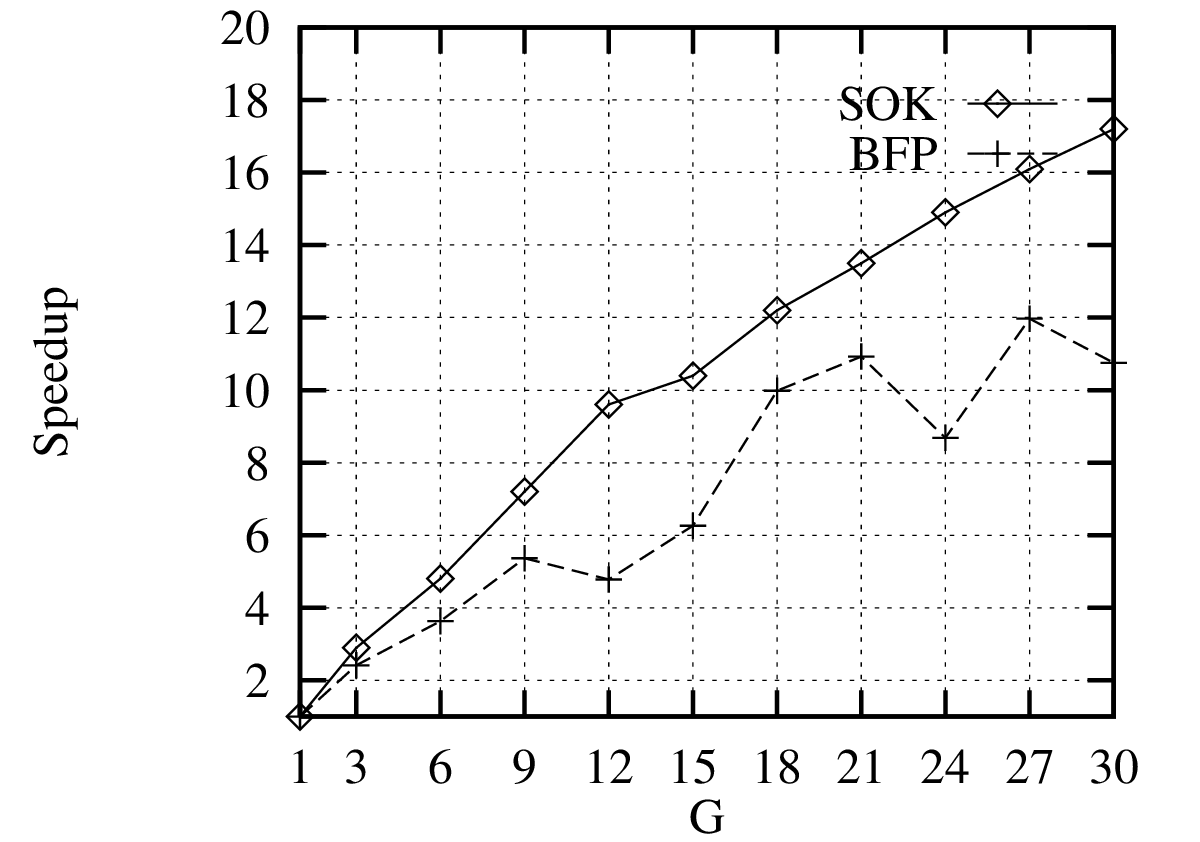
\includegraphics[width=\linewidth]{pent_sok.png}
  \caption{Speedup achieved for Pentominoes program with work splitting.}
  \label{pent_sok}
\end{figure}

The new approach addresses each of the following issues:
\begin{itemize}
\item{\textbf{Small poisoned oracles:} fundamental to the use of \texttt{kappa}
  for breadth-first partitioning is the generation of a large number of ports at
  each incremental depth limit, such that a path processor will rapidly process
  the ports with small subtrees and move on without requiring further communication
  with a control processor or further interruption of busy processors.}
\item{\textbf{Large poisoned oracles:} the interruption and splitting of the work of 
  busy path processors means that the SOK technique is not vulnerable to the
  unequal distribution of work that affects BFP.}
\item{\textbf{Selection of an appropriate depth limit:} the SOK strategy is effective
  with an initial depth limit of 1, such that initially only one path processor
  receives work with the others idle, and splitting repeatedly occurs until
  the work is allocated to all available path processors.}
\item{\textbf{Low communications requirements:} to minimise the communication
  overhead the frequency of communication and the quantity of data transferred
  on each split must be kept to a minimum.  Splitting with oracles and kappa
  reduces the frequency of communication by assigning multiple subtrees for
  search (at the incremental depth limit) on each assignment.  The oracle and
  the parameters of the breadth-first partitioning phase provide a very
  compact means of communicating the work required.}
\item{\textbf{Recovery from path processor failure:} the work assigned to a path
  processor is defined by the oracle and partitioning parameters.  The information
  can be communicated to an alternative processor for the search to be repeated.
  Annotation of solutions with the associated current oracle provides a simple
  mechanism to avoid duplicates.  The ease of recovery from
  processor failure using oracles extends the utility of the SOK strategy for
  large networks of general purpose workstations.}
\item{\textbf{Control processor requirements:} the SOK strategy described above
  suggests the use of a control processor to initiate the work and provide global
  control for scheduling.  The splitting technique described uses information local
  to the interrupted busy processor such that distributed or hierarchical
  control could equally be implemented, leaving the control processor to provide the
  user interface and startup and terminate execution.}
\end{itemize}

%%%%%%%%%%%%%%%%%%%%%%%%%%%%%%%%%%%%%%%%
\section{Extra-logical considerations} %
%%%%%%%%%%%%%%%%%%%%%%%%%%%%%%%%%%%%%%%%

The approach described in this paper is incompatible with the use of Prolog's
extra-logical predicates \textit{cut}, \textit{assert} and \textit{retract}.
A \textit{cut} discovered in the search tree of one path processor could imply
a pruning of subtrees already searched or in the process of search by others.
While oracles provide a basis for the communication of the discovery of a
\textit{cut}, analysis of existing Prolog code programs suggests that the
rapidity with which the cuts would be discovered in the search tree would cause
the overhead of communication to dominate the overall runtime \cite{Lew98}.

Deterministic procedures produce OR-only search trees with single entry and
exit points, such that oracle indexes within the procedure do not contribute
to OR-parallel speedup.  With oracle support removed from these procedures, the
OR-parallel behaviour of the program is unaffected.  This technique has been
used to provide limited support for \textit{cut} with the SOK strategy, with the
requirement that any procedure containing \textit{cut} must be deterministic.

The compiler \texttt{prologpf} developed at Cambridge implementing the
SOK strategy provides support for higher-order functional programming as an
alternative to the use of \textit{cut}.  No parallelisation is provided to
the evaluation of functions or
deterministic procedures containing \textit{cut}.  The interpretation of the
functional evaluation as a tree reduction process may provide an opportunity for
the extension of the oracles into the functional code, but this is an area for future
work.

%%%%%%%%%%%%%%%%%%%%%%%%%%
\section{Implementation} %
%%%%%%%%%%%%%%%%%%%%%%%%%%
\label{implementation}

Oracle management and partitioning support can be added to a standard Prolog
program through the use of a simple extra-logical predicate, \texttt{kappa}.

The sample program illustrated earlier in this paper can be transformed to use
\texttt{kappa} as follows, with the predicate inserted as the first subgoal in
the body of each clause:
\begin{verbatim}
% original program           % transformed program
g(U,V) :- p(U),q(V),r(U,V).  g(U,V) :- kappa(1),p(U),q(V),r(U,V).

p(1).                        p(1) :- kappa(1).
p(2).                        p(2) :- kappa(2).

q(1).                        q(1) :- kappa(1).
q(2).                        q(2) :- kappa(2).
\end{verbatim}
Assuming an array \texttt{oracle[1\ldots MAXORC]} to hold an oracle to be followed
of length \texttt{oracle\_{}length},
indexed by the current depth in a global variable \texttt{depth}, the search of the
program can be limited to the subtree defined by that oracle
with\footnote{The body of each \texttt{kappa} clause should be read as a
pseudo-code similar to 'C'.}:\\
\begin{tabular}{l l l}
\texttt{kappa(I)} & \texttt{:-} & \texttt{++depth;} \\
 & & \textit{if (}\texttt{depth}$\le$\texttt{oracle\_{}length}\textit{)}\\
 & & \textit{then if (}\texttt{I}$\ne$\texttt{oracle[depth]}\textit{)}\\
 & & \textit{~~~~~~then} \texttt{fail.}\\
 & & \textit{else} \texttt{oracle[depth] = I.}\\
\texttt{kappa(\_{})} & \texttt{:-} & \texttt{--depth; fail.} \\
\end{tabular}

This definition of \texttt{kappa} will also accumulate the current
oracle as an extension of the initial oracle given to be followed.  On
interruption, the current oracle can be returned by a signal handling
procedure or through the use of the standard Prolog \texttt{catch}
relation.  Constraining the search to the right of an oracle requires
the use of arithmetic comparison rather than equality, and takes
advantage of the ordering of the indexes of the clauses of each source
procedure.

Constraining the search of path processor \texttt{N} within a processor group of size \texttt{G}
to a subset of the subtrees at a selected depth \texttt{L}
can be achieved with the following definition of \texttt{kappa}:\\
\begin{tabular}{l l l}
\texttt{kappa} & \texttt{:-} & \texttt{++depth;} \\
 & & \textit{if (}\texttt{depth}$==$\texttt{L}\textit{)}\\
 & & \textit{then \{} \texttt{++port\_{}count;}\\
 & &           \textit{~~~~~~~~~if (}\texttt{port\_{}count mod G}
                   $\ne$ \texttt{N}\textit{) then} \texttt{fail}\\
 & &           \textit{~~~~~~~\}}.\\
\texttt{kappa} & \texttt{:-} & \texttt{--depth; fail.} \\
\end{tabular}

Note that partitioning from the root using \texttt{kappa} does not
require oracle support and the oracle index \texttt{I} in the previous
definition is not used.  The one-time breadth-first partitioning
described in this paper can be implemented with just this second
simple definition of \texttt{kappa}.  Work splitting can be
implemented with a combination of both definitions given plus a
procedure to return the current oracle on interruption.  The
treatment of \texttt{kappa} as an extra-logical predicate illustrates
the principle and provides a portable implementation with an overhead
typically of 10\% on a single cpu.  More efficient program
transformations are possible, and the support provided by
\texttt{kappa} could equally be embedded within the WAM call and
return instructions.

%%%%%%%%%%%%%%%%%%%%%%%%%%%%%
\section*{Acknowledgements} %
%%%%%%%%%%%%%%%%%%%%%%%%%%%%%

This research was supported in part by the Engineering and Physical
Sciences Research Council, and benefited from the
supervision of William Clocksin.

%%%%%%%%%%%%%%%%%%%%%%%%%%%%%
\begin{thebibliography}{99} %
%%%%%%%%%%%%%%%%%%%%%%%%%%%%%

\bibitem{Ali87}
K. A. M. Ali.
\newblock {OR}-parallel execution of {P}rolog on a Multi-Sequential Machine.
\newblock {\it Intl. Journal of Parallel Programming}, {\bf 15}(3):189--214, 1987.

\bibitem{Bea91}
A. Beaumont.
\newblock Scheduling strategies and speculative work.
\newblock In {\it Parallel Execution of Logic Programs}, Beaumont and Gupta (Eds),
          Springer Verlag, 120--131, 1991.

\bibitem{B+92}
J. Briat et al.
\newblock {OPERA}: {OR}-parallel {P}rolog System on Supernode.
\newblock In {\it Implementations of Distributed {P}rolog}, Kacsuk and Wise (Eds),
           Wiley, 1992.

\bibitem{BDLO+88}
R. Butler, T. Disz, E. Lusk, R. Olson, R. Overbeek and R. Stevens.
\newblock Scheduling {OR}-parallelism: an {A}rgonne perspective.
\newblock {\it Proc. Fifth Intl. Conf. and Symposium on Logic Programming}, 
          MIT Press, 1590--1605, 1988.

\bibitem{Clo87}
W.~F. Clocksin.
\newblock Principles of the {D}el{P}hi Parallel Inference Machine.
\newblock {\it Computer Journal}, {\bf 30}:386--392, 1987.

\bibitem{Clo92}
W.~F. Clocksin.
\newblock The {D}el{P}hi Multiprocessor Inference Machine.
\newblock {\it Proc. 4th U.K.\ Conf.\ on Logic Programming}, K.~Broda (Ed),
           Springer-Verlag, 189--198, 1992.

\bibitem{DLO87}
T. Disz, E. Lusk and R. Overbeek.
\newblock Experiments with {OR}-parallel logic programs.
\newblock In {\it Proc. of the 4th Intl. Conf. on Logic Programming},
          {\bf 2}:576--600, MIT Press, 1987
	
\bibitem{Lew98}
Ian~J.~Lewis.
\newblock PrologPF: Parallel logic and functions on the {D}elPhi {M}achine.
\newblock {\it PhD Thesis}, Computer Lab, Cambridge University, England, 1998. 

\bibitem{LWH+90}
E. Lusk and D. H. D. Warren and S. Haridi et al.
\newblock The {A}urora OR-parallel {P}rolog system.
\newblock {\it New Generation Computing}, {\bf 7}:243--271, 1990.
	
\bibitem{Sar95}
S.~Saraswat.
\newblock Performance evaluation of the DelPhi Machine.
\newblock {\it PhD Thesis}, Computer Lab, Cambridge University, England, 1995.

\bibitem{Sti88}
M.~Stickel.
\newblock A {P}rolog technology theorem prover:
          {I}mplementation by an extended {P}rolog
          compiler.
\newblock {\it J. Auto. Reasoning}, {\bf 4}(4):353--380, 1988.
	
\bibitem{War87}
D. H. D. Warren.
\newblock The {SRI} model for OR-Parallel execution of {P}rolog - Abstract
          design and implementation issues.
\newblock In {\it Proc. Symposium on Logic Programming}, 46--53,
          IEEE Computer Society Press, 1987.

\end{thebibliography}

\end{document}
